\newchapter{Musket Ball: DM Implications}{Musket Ball Cluster: Dark Matter Implications}{Musket Ball Cluster: Dark Matter Implications}
\label{chapter:4}

\noindent Portions of this chapter were originally published in the article titled \emph{Discovery of a Dissociative Galaxy Cluster Merger with Large Physical Separation} which was published in the March 2012 issue of the Astrophysical Journal Letters (Volume 747, pp. L42). \\

Chapter abstract text

\section{Introduction}



Intro text \citep{Dawson:2012dl}

\subsection{Location Estimation}
For the original work of \citet{Dawson:2012dl} (see Chapter 2) I estimated the weak lensing subcluster positions and errors on their positions by using the location of the peak signal in a region and estimated the variance on the peak by measuring the peak location of each bootstrap iteration within the selected region.  
For this chapter, rather than using the location of the peak and variance of the peak, I have adopted an iterative centroid estimation scheme, similar to \citet{Randall:2008hs}. 
I begin by calculating the centroid of a large aperture that encompasses one subcluster, but excludes the other.
I then decrease the aperture, recenter on the previously calculated centroid, and estimate the centroid of the new aperture.
This process is repeated until the aperture is decreased to a radius of XXX kpc.
To estimate the uncertainty on the location I perform this process on each iteration of a random bootstrap sample map, resulting in a array of centroid values.
 The uncertainty on the location is then inferred from the variance of this array of centroid values.


%-------------------------------------------------------
%-------------------------------------------------------
%-------------------------------------------------------
\section{Galaxy Location}

since the spec-z errors are typically of order XXX km/s their probability distribution can be treated as a delta function.

% Donimant components of unceartainty

two dominant components to the uncertainty: 1) Poisson noise, simply attempting to measure a global property (center of the galaxy distribution) with a discrete number of samples, 2) systematic error due to cluster membership uncertainty

Information for determining membership is limited to spectroscopic and photometric redshift information

Difficult to obtain spectroscopic redshifts for a large number of galaxies and often limited to magnitudes R<23. Reasons why hard...
Easier to obtain photometric redshifts for a large number of galaxies, compare the sample magnitude distribution of galaxies in the area of a spectroscopic survey of the Musket Ball Cluster (Figure \ref{figure:PhotozSpeczMagDist}).
However photomety errors increase for fainter galaxies and this in turn increases the photometric redshift uncertainty.  For the DLS it is found that the photo-z's become unreliable fainter than $R\sim$24 \citep{Schmidt:2013ig}.

\begin{figure}
	\centering
	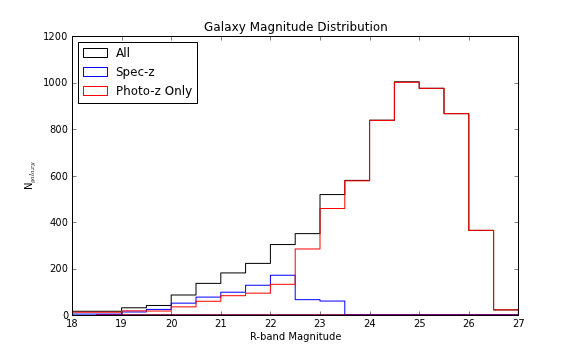
\includegraphics[width=5in]{Chapter4/AnalysisFiles/magdist.png}
	\caption[Musket Ball Cluster spectroscopic and photometric magnitude distribution.]{Gives some idea of the galaxy sample magnitude distribution. DLS photometry.
		}
	\label{figure:PhotozSpeczMagDist}
\end{figure}

There is a balancing act between these two components of the uncertainty

The systematic error due to contamination can be decreased by placing strict membership requirements, e.g. only using galaxies that have spectroscopic redshifts within some small factor (e.g. 3) of the cluster velocity dispersion.
However this will reduce the number of galaxies that are used to estimate the centroid and the Poisson noise will increase.
Conversely...

Bootstrap method should account for both of these error components.

We consider two different methods of membership identification...

\subsubsection{Fully Probabilistic Membership Determination}

This method is rooted in the desire to treat both samples in a consistent manner.


\begin{equation}
w(draw)_i = \int_{0}^{\infty} p(z)_i \frac{1}{\sigma_{\rm vdisp}\sqrt{2\pi}}e^{\frac{-(z-z_{\rm cluster})^2}{2\sigma_{\rm vdisp}^2}}\mathrm{d}z
\label{equation:specz_weight}
\end{equation}

\begin{equation}
w(draw)_i = \int_{0}^{\infty} \frac{1}{\sigma_{\rm z-phot_{i}}\sqrt{2\pi}}e^{\frac{-(z-z_{\rm phot_{i}})^2}{2\sigma_{\rm z-phot_{i}}^2}} \frac{1}{\sigma_{\rm vdisp}\sqrt{2\pi}}e^{\frac{-(z-z_{\rm cluster})^2}{2\sigma_{\rm vdisp}^2}}\mathrm{d}z
\label{equation:photoz_weight}
\end{equation}

\begin{equation}
\sigma_{\rm z-phot_{i}} \approx \bar{\sigma}(1+z_{\rm phot_{i}})
\label{equation:SigmazPhot}
\end{equation}



\begin{figure}
\centering
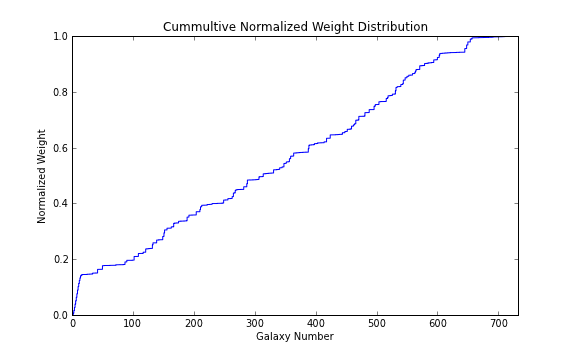
\includegraphics[width=5in]{Chapter4/AnalysisFiles/cumnormwghtdist.png}
\caption[Probabilistic scheme; cumulative normalized weight distribution for galaxies being in the Musket Ball Cluster.]{
This weight distribution is used to perform a weighted random draw of cluster galaxies.
This distribution is determined by Equations \ref{equation:specz_weight} and \ref{equation:photoz_weight}.
During the bootstrap sampling process a random number between 0 and 1 is drawn from a uniform distribution, where this random number intersects the weight distribution determines the randomly selected galaxy.
Note that the catalog is sorted such that the spectroscopic members are first, thus the noticeably steeper slope for the early galaxy numbers.
}
\label{figure:NormWeightDist}
\end{figure}

\begin{figure}
\centering
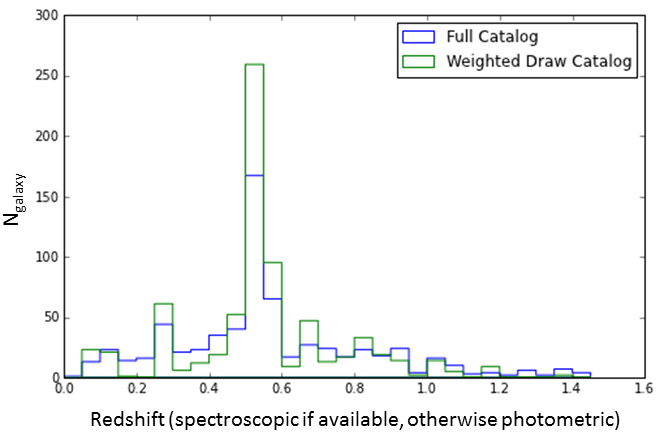
\includegraphics[width=5in]{Chapter4/AnalysisFiles/zdist_randomweightdraw_reformat.png}
\caption[Comparison of parent galaxy redshift distribution with weighted random draw distribution.]{

}
\label{figure:ProbWeightDist}
\end{figure}

\subsubsection{Hard Redshift Bounds}
Hard redshift cut... why? 1) we are more concerned with purity 

Spectroscopic galaxies should not really be penalized 


spec-z bounds, and justification

photo-z bounds, and justification

photo-z normalization

\textbf{Normalizing based on overlapping probability distribution functions...}

\begin{equation}
w(draw)_i = \frac{\int_{0}^{\infty} \frac{1}{\sigma_{\rm z-phot_{i}}\sqrt{2\pi}}e^{\frac{-(z-z_{\rm phot_{i}})^2}{2\sigma_{\rm z-phot_{i}}^2}} \frac{1}{\sigma_{\rm vdisp}\sqrt{2\pi}}e^{\frac{-(z-z_{\rm cluster})^2}{2\sigma_{\rm vdisp}^2}}\mathrm{d}z}{\int_{0}^{\infty} \frac{1}{\sigma_{\rm z-phot}(z_{\rm cluster})\sqrt{2\pi}}e^{\frac{-(z-z_{\rm cluster})^2}{2\sigma_{\rm z-phot}(z_{\rm cluster})^2}}\frac{1}{\sigma_{\rm vdisp}\sqrt{2\pi}}e^{\frac{-(z-z_{\rm cluster})^2}{2\sigma_{\rm vdisp}^2}}\mathrm{d}z}
\label{equation:NormalizedPhotozWeight}
\end{equation}

Note that because of the dependence of $\sigma_{\rm z-phot_{i}}$ on $z$, see Equation \ref{equation:SigmazPhot}, the maximum photometric weight actually occurs at a redshift slightly lower than the cluster redshift. For the case of the Musket Ball redshift $z=0.53$ and $\bar{\sigma}=0.07$ the maximum occurs at $z=0.523$. We will not bother to go into these details since we will argue for a more appropriate weighting scheme.

\textbf{Normalizing based on empirical data}

Photo-z Penalization Factor

This penalization factor is based in the fact that from our magnitude limited survey\footnote{The survey was magnitude limited in regards to the fact that we targeted any galaxy with $R$<23.5, if galaxies had a 0.43$\leq z_{\rm phot} \leq$0.63 there likelihood of being target was twice that of other galaxies. This should not bias the conclusions of this section since we are limiting ourselves to considering just the range 0.43$\leq z_{\rm phot} \leq$0.63. Figure \ref{figure:PhotozSpeczMagDist} shows the approximate completeness of this survey.} (R<23.5) of the Musket Ball we targeted 355 galaxies between 0.43= 3) and 210 of these spectra were between 0.525<specz<0.54 (with quality>=3), see for example the figure below. This translates to a sample purity of 63\%.  Thus I will multiply all of the photo-z galaxy weights by a penalization factor of 0.63.


\begin{figure}
\centering
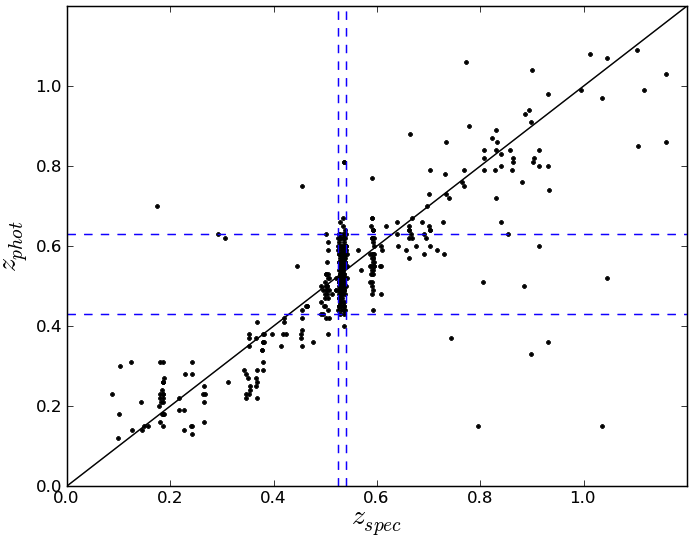
\includegraphics[width=5in]{Chapter4/photVSspec.png}
\caption[Spectroscopic verses photometric redshift for the Musket Ball Cluster.]{

}
\label{figure:photzVSspecz}
\end{figure}

\begin{figure}
\centering
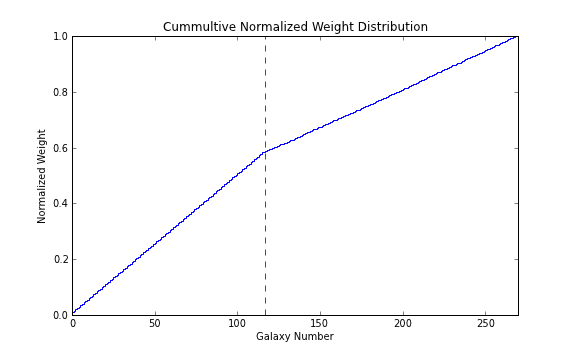
\includegraphics[width=5in]{Chapter4/AnalysisFiles/cumnormwghtdist_zclip_photozpenalty.png}
\caption[Photometric redshift penalization scheme; cumulative normalized weight distribution for galaxies being in the Musket Ball Cluster.]{
}
\label{figure:NormPenaltyWeightDist}
\end{figure}


%\begin{figure}
%\centering
%\includegraphics[width=5in]{ }
%\caption[]{
%}
%\label{}
%\end{figure}

\subsection{Galaxy Location Results}

Perhaps include a table with the actual coordinates and confidence limit values.

\begin{figure}
\centering
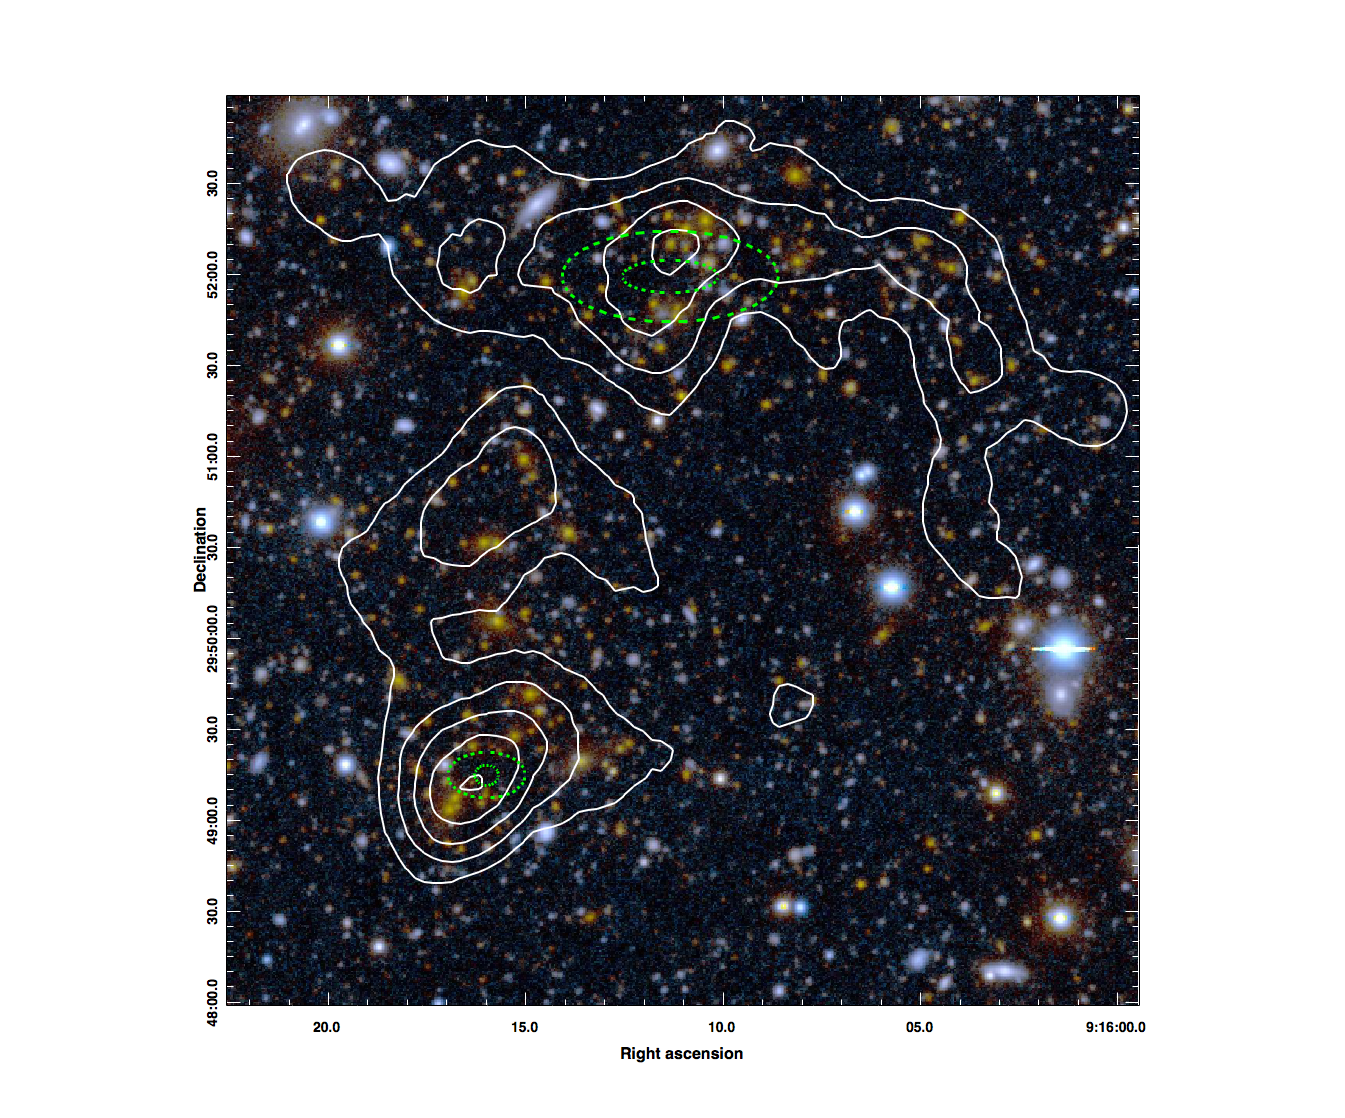
\includegraphics[width=5in]{Chapter4/DLScolor_wGalDenCon.png}
\caption[Musket Ball Cluster galaxy number density map including spectroscopic redshift information.]{
DLS composite $BVR$ color image of the Musket Ball Cluster showing  the galaxies of the two subclusters (predominately orange). 
This figure is similar to Figure \ref{fig2}, however the white contours representing the number density of galaxies now include both spectroscopic and photometric redshift information.
All (117) with galaxies spectroscopic redshift within three times the velocity dispersion of each subcluster were given a weight of 1.
All (270) galaxies without a spectroscopic redshift but with $z_{\rm phot}=0.53\pm0.1$ (the cluster redshift $\pm\sigma_{z_{\rm phot}}$) were given a weight of 0.63.
The photometric redshift sample weight is based on the empirically determined cluster membership purity of this sample, as determined from our magnitude limited spectroscopic survey of the cluster.
The contours begin at $\sim$200 galaxies\,Mpc$^{-2}$ with increments of $\sim$50 galaxies\,Mpc$^{-2}$.
The dashed green ellipses show the approximate galaxy centroid 68\% and 95\% confidence limits for each subcluster.
}
\label{figure:GalDenMap_withspec}
\end{figure}


%--------------------------------------------------------
%--------------------------------------------------------
%--------------------------------------------------------
\section{Gas Location}

When estimating the central gas centroid (black circles of Figure \ref{figure:XrayCentroid}), all detected point sources (small green circles with red dashes of Figure \ref{figure:XrayCentroid}) are excluded.
Additionally the diffuse southern gas concentration is excluded (large green rectangular box of Figure \ref{figure:XrayCentroid}).
The remaining X-ray photons in the green semicircle are then used to estimate the gas centroid of the central concentration, using  the \textit{dmstat} function of the Chandra Interactive Analysis of Observations (CIAO) software package.
We note that adaptive smoothing can introduce some artifacts to the image, however we find excellent agreement between the centroid of the smoothed image (black `x' in Figure \ref{figure:XrayCentroid}) and the centroid of the unsmoothed image (black circles of Figure \ref{figure:XrayCentroid}) suggesting that the smoothed map provides a reasonable representation of the gas.

We find that the central gas concentration centroid ($09\fh16\fm13\fs\pm8\fs, 29\fdg50\farcm55\farcs\pm9\farcs$) is offset $5.0\farcs$ from the peak of the gas distribution ($09\fh16\fm15\fs\pm5.5\fs, 29\fdg50\farcm59\farcs\pm5.0\farcs$).
Both are significantly offset between the northern and southern galaxy and WL concentrations.

\begin{figure}
\centering
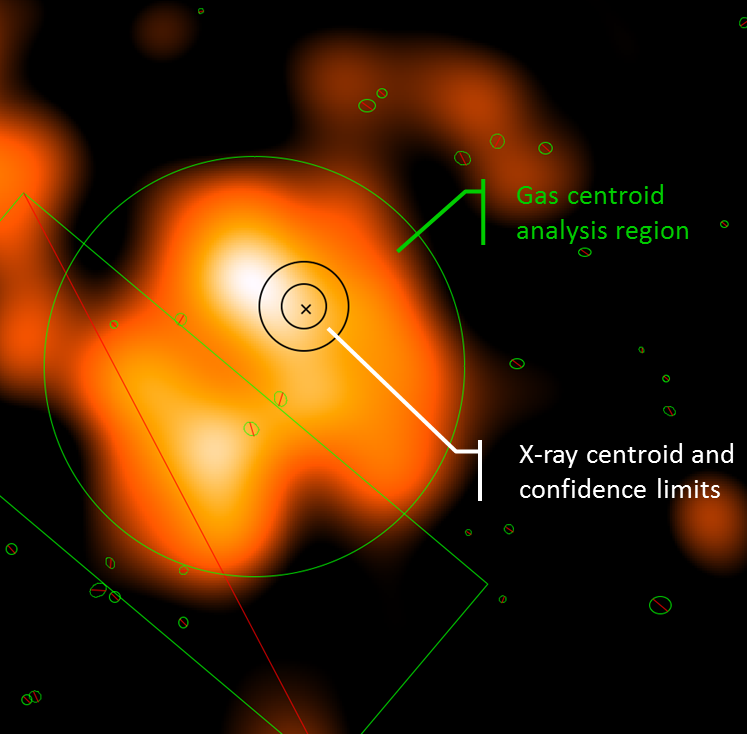
\includegraphics[width=5in]{Chapter4/XrayCentRegions_reformat.png}
\caption[Musket Ball Cluster X-ray map with estimated centroid.]{
Chandra ACIS-I 40\,ks adaptively smoothed X-ray image of DLSCL J0916.2+2951 (the same as Figure \ref{figure:MusketBallXray}).
The green circles and boxes are the SAOImageDS9 inclusion and exclusion regions used in conjunction with the Chandra Interactive Analysis of Observations (CIAO) software package.
The unsmoothed central gas centroid 68\% and 95\% confidence intervals are represented by the black circles.
The smoothed central gas centroid is represented by the black `x'.
The image field-of-view is the same as Figure \ref{fig1}.
}
\label{figure:XrayCentroid}
\end{figure}

%-------------------------------------------------------
%-------------------------------------------------------
%-------------------------------------------------------

\section{Weak Lensing Location}

\subsubsection{Noise and Systematic effects}

\textit{Copied from Chandra/HST proposal. Need to edit.}

Several sources of noise and systematic effect could cause such an offset:
(1) the mass of the northern subcluster pulling off the overall mass
centroid; (2) the gas mass just to the north doing the same; and (3)
unrelated structures along the line of sight. We show below that (2)
is the primary concern and can be solved with Chandra data, and that
(4) HST data are required to tighten up the statistical uncertainty on
the size of offset.  Together, these data will enable measurement of
$\sigma_{\rm DM}m_{\rm DM}^{-1}$.

\textbf{(1)} We model the surface mass density of the north and south subclusters with three NFW halos using masses determined by \citet{Dawson:2012dl}. We recursively estimate the centroid of this model and find an offset $3.4''$ from the true centroid towards the northern subcluster. 
\textbf{(2)} We then combine estimated surface mass densities of the
Central and South gas concentrations with the previous DM surface
densities from step (1) which results in a $7.6''$ centroid offset (dashed red curve of Figure \ref{fig3}).  
For perspective, if we double the gas mass the total offset increases to $10''$, or if we account for the uncertainty in our distribution of the gas mass the modeled centroid offset ranges from $3.4''$ to $9.4''$ (light red region of Figure \ref{fig3}). 
With the proposed Chandra observations we can better constrain the gas mass by approximately a factor of 10 and constrain the distribution of the gas mass so that the resulting uncertainty in the modeled centroid offset is reduced by at least a factor of 2 (dark red region of Figure \ref{fig3}).
\textbf{(3)} As discussed in \citet{Dawson:2012dl} we find no evidence of significant line of sight structures using our full sample of 654 spectroscopic redshifts (with uniform selection over $0<z<1.0$) as well as photometric redshifts. 
Based our findings we confidently rule out any line of sight structures with $M_{\rm 200}\gtrsim1\times10^{12} M_\odot$; any undetected structure will have negligible impact on the offset.
\textbf{(4)} We estimate the noise of the galaxy density and weak lensing centroids by performing the recursive centroid analysis on bootstrap samples of each.
For the galaxy density centroid errors we take 1000 bootstrap samples of the spectroscopically confirmed cluster galaxies and remaining galaxies with $0.43<z_{\rm phot}<0.63$ (roughly the cluster redshift $\pm\sigma_{z_{\rm phot}}$).
Similarly we estimate the weak lensing centroid errors by analyzing 1000 bootstrap samples of the lensed background galaxies.

\section{Gas--Weak Lensing Offset}

%copied from \citep{Dawson:2012dl}
The peak of the gas distribution ($09\fh16\fm15\fs\pm5.5\fs, 29\fdg50\farcm59\farcs\pm5.0\farcs$) derived from X-rays is offset $1.4\arcmin\pm0.49$ from the North HST WL mass peak ($09\fh16\fm10\fs\pm30\fs, 29\fdg52\farcm10\farcs\pm30\farcs$), and $1.4\arcmin\pm0.14$ from the South HST WL mass peak ($09\fh16\fm15\fs\pm8.0\fs, 29\fdg49\farcm34\farcs\pm6.9\farcs$), and is located near a local minimum in the mass (see Figure \ref{fig3}).
Given the significant offset between the WL and gas locations we are able to use the first method of \citet{Markevitch:2004dl} and place a rough limit on the DM self-interaction cross-section, $\sigma_{\rm DM}$.
This method compares the scattering depth of the dark matter, $\tau_{\rm DM}=\sigma_{\rm DM}m^{-1}_{\rm DM} \Sigma_{\rm DM}$, with that of the ICM gas, $\tau_{\rm ICM}\approx 1$, where $m_{\rm DM}$ is the DM particle mass and $\Sigma_{\rm DM}$ is the surface mass density of the DM particles.
$\Sigma_{\rm DM}$ is approximately the WL measured surface mass density, $\Sigma$, since $\sim80\%$ of a typical cluster's mass is DM \citep{Diaferio:2008js}.
For ease of comparison with the results of \citet{Markevitch:2004dl} and \citet{Merten:2011gu} we examine the surface density averaged over the face of the subcluster within $r$=125\,kpc, which is $\Sigma\approx0.15$\,g\,cm$^{-2}$; thus we find $\sigma_{\rm DM} m_{\rm DM}^{-1} \lesssim 7$\,cm$^2$\,g$^{-1}$.  
Note that we cannot apply the velocity-dependent $\sigma_{\rm DM}$ constraint methods outlined by \citet{Markevitch:2004dl} since our analytic model assumes $\sigma_{\rm DM}$\,=\,0 \citep{Dawson:2012dl, Dawson:2012ub}.



\begin{figure}
%\plottwo{fig3a.eps}{fig3b.eps}
\plotone{Chapter2/fig3.png}
\caption[Comparison of the Subaru $i'$-band ground-based and HST space-based WL mass signal-to-noise maps of DLSCL J0916.2+2951 with the X-ray distribution and galaxy number density.]{Comparison of the Subaru $i'$-band ground-based (left) and HST space-based (right) WL mass signal-to-noise maps (color) of DLSCL J0916.2+2951 with the X-ray distribution (bold black contours) and galaxy number density (white contours, same as Figure \ref{fig2}). The peak centers and corresponding one sigma errors are denoted by the gray cross-hairs.
In both analyses there is agreement between the location and relative magnitude of galaxies and WL yet the majority of the cluster gas is centered $\sim1.4\arcmin$ between the North and South subclusters in a local mass underdensity, providing evidence that the North and South subclusters have undergone the first pass-through of a major merger.
The scale of each map is equivalent and the image field-of-view is the same as Figures \ref{fig1} \& \ref{fig2}.
The map created from the joint Subaru/HST catalog looks nearly identical to the HST map, with only slight variations in the scale (see Table \ref{tbl1}).
\label{figure:SubaruHSTwlComparison}}
\end{figure}

\section{Galaxy--Weak Lensing Offset}

Section text

%-----------------------------Figure Start------------------------------
% Single panel figure
\begin{figure}[t]
	\centering
	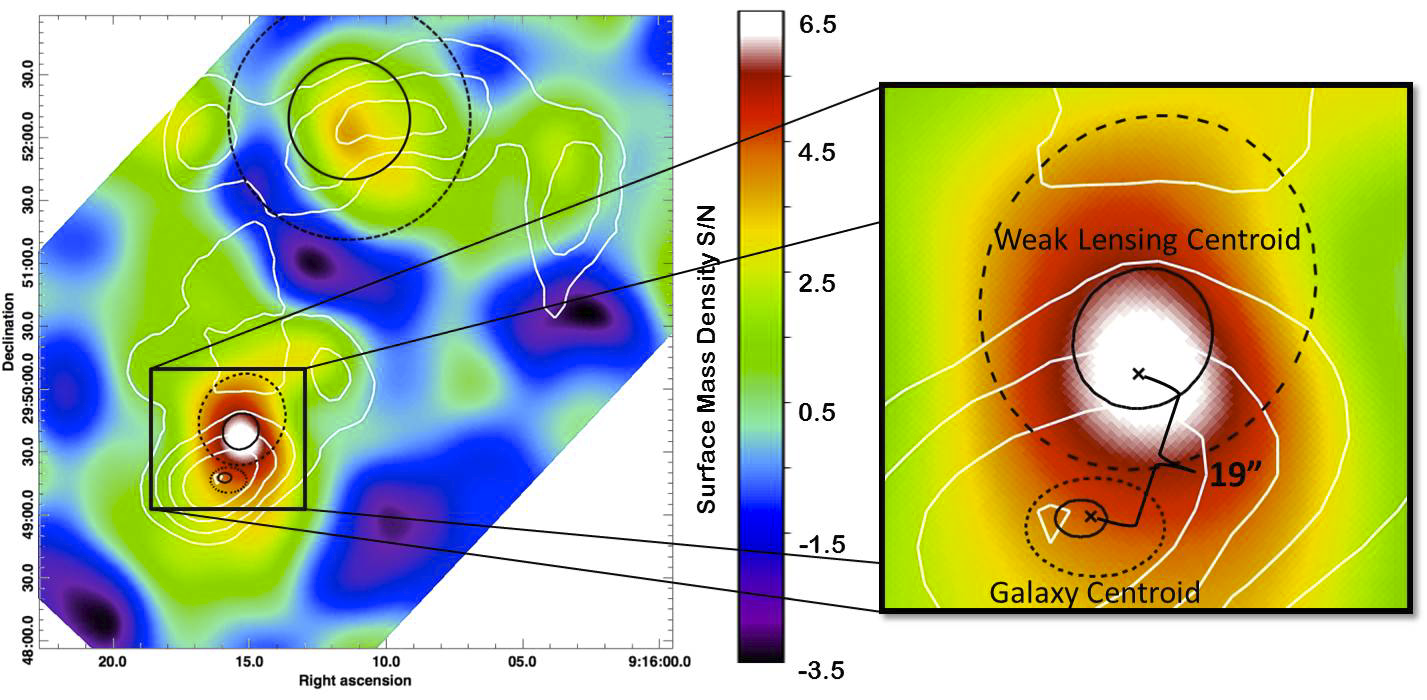
\includegraphics[width=6in]{Chapter4/WLgalaxyoffset.png}
	\caption[Musket Ball Cluster galaxy-weak lensing offset.]{
		\small{The WL mass signal-to-noise map based on HST measured shapes is shown in color with the galaxy number density isopleths in white.  
		The inset shows the 68\% (solid black) and 95\% (dashed black) confidence intervals on the South subcluster's WL and galaxy density centroids.  
		We have detected a 19" offset between the galaxies and the WL mass in the South subcluster that is consistent with the offset expected if DM has a non-zero cross-section just below the current published upper limits.  
		This is the best astrophysical evidence to date of a non-zero DM cross-section.  While a consistent offset is observed for the North subcluster, the large WL centroid error prohibits measurement of a significant offset for that subcluster.
		}
	}
	\label{figure:galaxyWLoffsetZoom}
\end{figure}
%-----------------------------Figure End--------------------------------

\begin{figure}
\centering
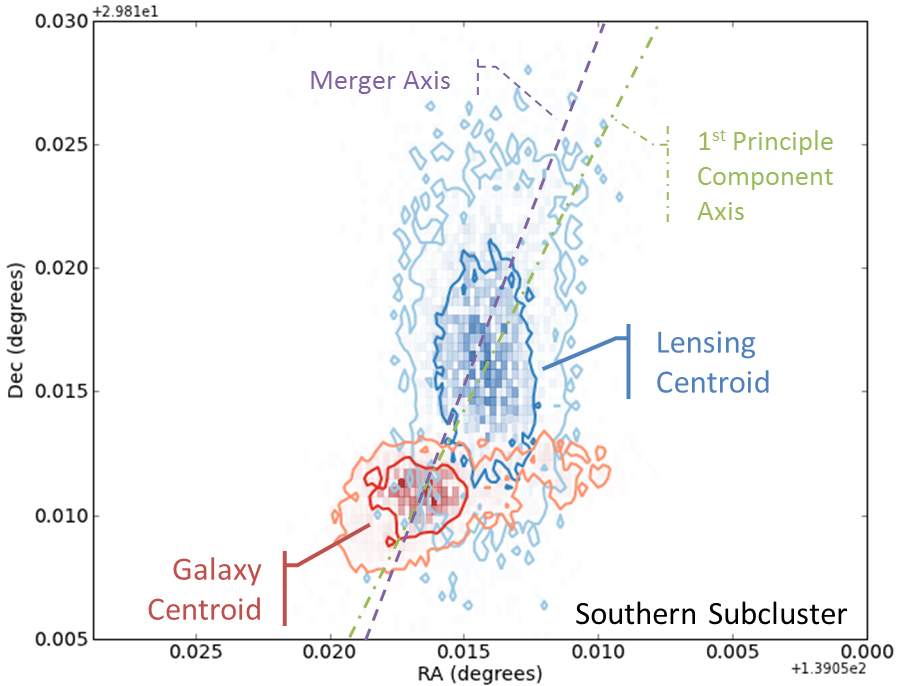
\includegraphics[width=5in]{Chapter4/AnalysisFiles/southcentroids_histplot2d_reformat.png}
\caption[Musket Ball southern subcluster galaxy and weak lensing centroid spatial distribution.]{
1.5' by 1.5'
Merger axis position angle = 159 degrees
First Principle component axis position angle =  153 degrees
}
\label{figure:CentroidDist_South}
\end{figure}

\begin{figure}
\centering
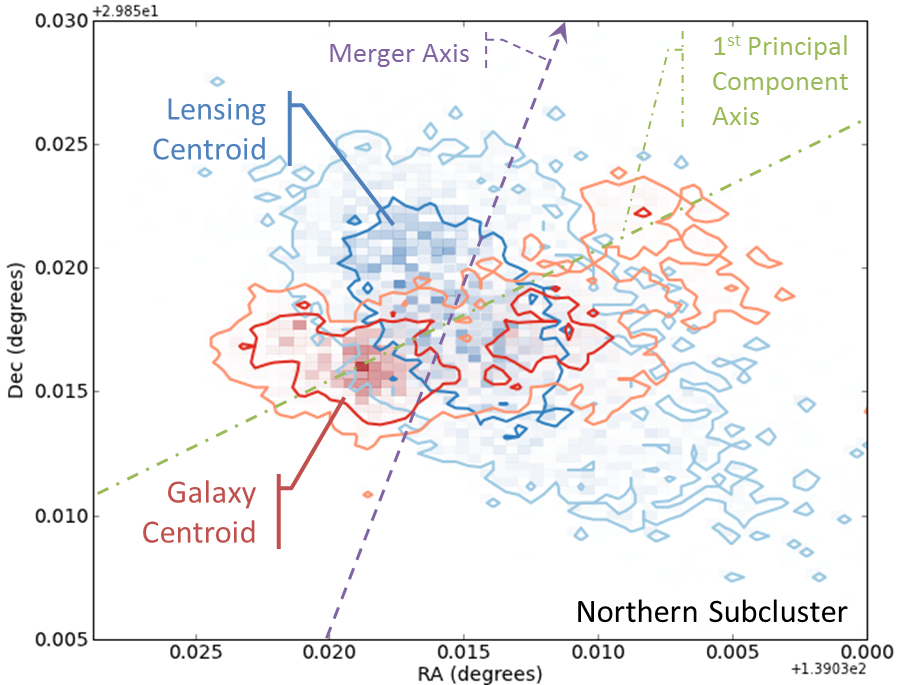
\includegraphics[width=5in]{Chapter4/AnalysisFiles/northcentroids_histplot2d_reformat.png}
\caption[Musket Ball northern subcluster galaxy and weak lensing centroid spatial distribution.]{
1.5' by 1.5'
}
\label{figure:CentroidDist_North}
\end{figure}

Perhaps include some figures discussing systematic offset tests.


\begin{figure}
\centering
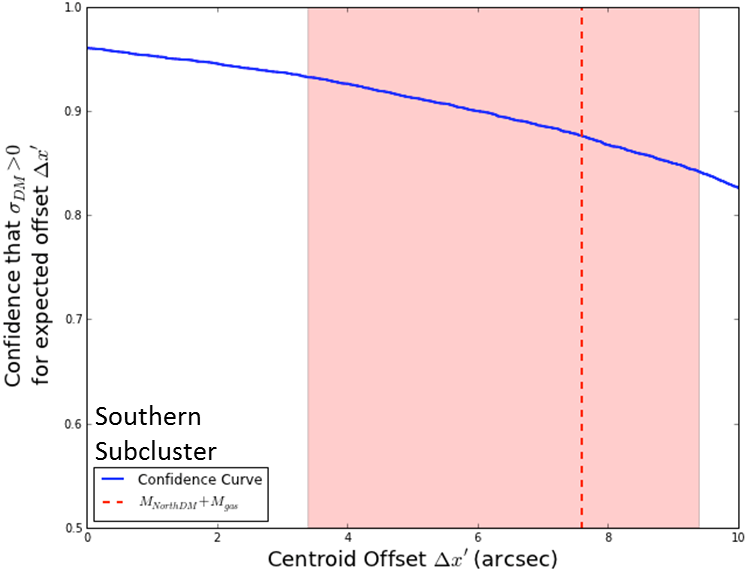
\includegraphics[width=5in]{Chapter4/AnalysisFiles/GalDenVsHSTWL_pzpen_delxPC_south_reformat.png}
\caption[Musket Ball southern subcluster galaxy and weak lensing centroid offset significance.]{
}
\label{figure:CentroidSignificance_South}
\end{figure}

\begin{figure}
\centering
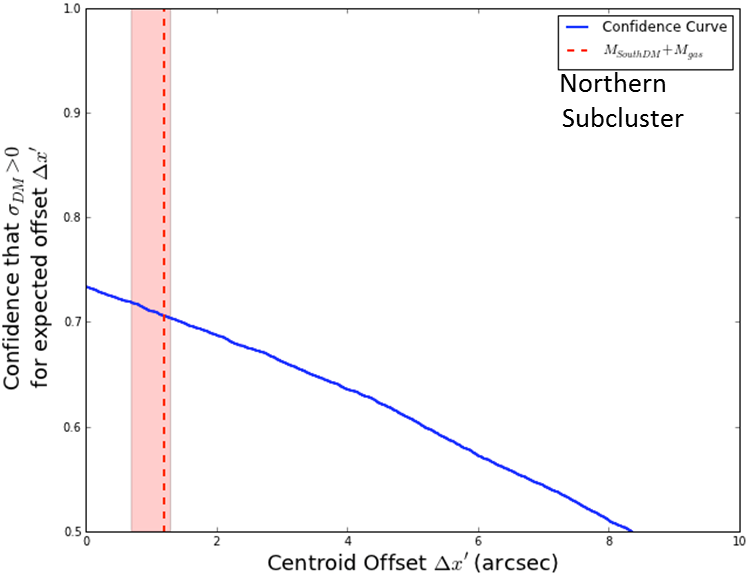
\includegraphics[width=5in]{Chapter4/AnalysisFiles/GalDenVsHSTWL_pzpen_delxPC_north_mergeraxis_reformat.png}
\caption[Musket Ball northern subcluster galaxy and weak lensing centroid offset significance.]{
}
\label{figure:CentroidSignificance_North}
\end{figure}

\section{Discussion}

Discussion text

note importance of fitting both subcluster simultaneously

better modeling of the gas mass and its effect on the systematic centroid offset

note alternatives to centroid estimation, both in measuring the galaxy-dark matter offset as well as just other ways to measure the galaxy centroid, e.g. \citep{Randall:2008hs}

For galaxy centroid consider other measurements of the galaxy population location, other than number density, for example weighting the galaxies by luminosity or stellar mass.

Discuss work of \citep{Kahlhoefer:2013wp}



\section{Conclusions}

Conclusion text

\textbf{acknowledgements:}
Acknowledgment text
%\end{acknowledgements}

%\bibliographystyle{apj}
%\bibliography{Chapter1/chapter1}{}



%% The References
%\bibliographystyle{thesis}
%\begin{singlespacing}
%  \bibliography{Chapter3/chapter3}
%\end{singlespacing}
